\section{Лекция 11}
\subsection{\S XVII.1. Квантовое описание тождественных систем.}
Напомним: когда локализация частиц со временем теряется, их нельзя различить. Рассмотрим две тождественные частицы:
\[
\xi_i = \{\vec{r}_i,~s_i\}, \tab \braket{\xi_1,~\xi_2}{\xi_1',~\xi_2'} = \delta(\xi_1 - \xi_1')\delta(\xi_2 - \xi_2').
\]
Оператор перестановки этих частиц:
\[
\hat{P}_{12}\ket{\xi_1,~\xi_2} = \ket{\xi_2,~\xi_1} = \pm\ket{\xi_1,~\xi_2}, \ \hat{P}_{12}^2 = \hat{1}
\]
Поговорим об описании такой системы в терминах волновых функций. У нас есть гильбертово пространство $\mathcal{H} = \mathcal{H}^{(1)}\otimes\mathcal{H}^{(2)}$, в котором живут тождественные частицы, пусть $\ket{\psi}\in\mathcal{H}$, $\psi(\xi_1,~\xi_2) = \braket{\xi_1,~\xi_2}{\psi}$. Как $\hat{P}_{12}$ действует в веденном нами базисе?
\[
\braupket{\xi_1,~\xi_2}{\hat{P}_{12}}{\psi} = \int d\xi_1'~d\xi_2'~\braupket{\xi_1,~\xi_2}{\hat{P}_{12}}{\xi_1',~\xi_2'}\braket{\xi_1',~\xi_2'}{\psi} = \int d\xi_1'~d\xi_2'~\braket{\xi_1,~\xi_2}{\xi_2',~\xi_1'}\psi(\xi_1',~\xi_2')
\]
Т.к. из условия нормировки $\braket{\xi_1,~\xi_2}{\xi_2',~\xi_1'} = \delta(\xi_1 - \xi_2')\delta(\xi_2 -\xi_2')$, получаем
\[
\braupket{\xi_1,~\xi_2}{\hat{P}_{12}}{\psi} = \pm \psi(\xi_2,~\xi_1)
\]
Во многих учебниках это "вульгарно" \ записывают как $\hat{P}_{12} \psi(\xi_1,~\xi_2) = \psi(\xi_2,~\xi_1)$.\\

С другой стороны, из свойств оператора перестановки следует
\[
\braupket{\xi_1,~\xi_2}{\hat{P}_{12}}{\psi} = \int d\xi_1'~d\xi_2'~\braupket{\xi_1,~\xi_2}{\hat{P}_{12}}{\xi_1',~\xi_2'}\braket{\xi_1',~\xi_2'}{\psi} = \pm \int d\xi_1'~d\xi_2'~\braket{\xi_1,~\xi_2}{\xi_1',~\xi_2'}\psi(\xi_1',~\xi_2') = \pm \psi(\xi_1,~\xi_2)
\]

Объединяя результаты, получим
\[
\psi(\xi_2,~\xi_1) = \pm\psi(\xi_1,~\xi_2)
\]
Это важное свойство, в дальнейшем свяжем эту симметрию/антисимметрию волновых функций со спином тождественных частиц.\\

Рассмотрим свойства оператора перестановки тождественных частиц.
\begin{enumerate}
	\item Эрмитовость: $\hat{P}_{12} = \hat{P}_{12}^\dagger$.
	\begin{proof}
		С учетом условия нормировки
		\[
		\delta(\xi_1 - \xi_2')\delta(\xi_2 - \xi_1') = \braket{\xi_1,~\xi_2}{\xi_2',~\xi_1'} = \bra{\xi_1,~\xi_2}\left(\hat{P}_{12}\ket{\xi_1',~\xi_2'}\right) = \braupket{\hat{P}_{12}^\dagger}{\xi_1,~\xi_2}{\xi_1',~\xi_2'} = \left(\braupket{\xi_1',~\xi_2'}{\hat{P}_{12}^\dagger}{\xi_1,~\xi_2}\right)^*
		\]
		Сопряжем обе части равенства и учтем четность дельта-функции:
		\[
		\braupket{\xi_1',~\xi_2'}{\hat{P}_{12}^\dagger}{\xi_1,~\xi_2} = \delta(\xi_1' - \xi_2)\delta(\xi_2' - \xi_1) = \braket{\xi_1',~\xi_2'}{\xi_2,~\xi_1} = \bra{\xi_1',~\xi_2'}\left(\hat{P}_{12}\ket{\xi_1,~\xi_2}\right)
		\]
		\[
		\Longrightarrow \ \hat{P}_{12}^\dagger = \hat{P}_{12}
		\]
	\end{proof}
	\item Унитарность: $\hat{P}_{12}\hat{P}_{12}^\dagger = \hat{P}_{12}^\dagger\hat{P}_{12} = \hat{1}$.
	\begin{proof}
		\[
		\begin{cases}
			\hat{P}_{12}^2 = \hat{1}\\
			\hat{P}_{12}\hat{P}_{12}^{-1} = \hat{P}_{12}^{-1}\hat{P}_{12} = \hat{1}\\
		\end{cases} \ \Longrightarrow \ \hat{P}_{12}^{-1} = \hat{P}_{12} \ \Longrightarrow \ \hat{P}_{12}^{-1} = \hat{P}_{12}^\dagger
		\]
		Значит, по определению обратного оператора, $\hat{P}_{12}\hat{P}_{12}^\dagger = \hat{P}_{12}^\dagger\hat{P}_{12}=\hat{1}$, т.е. оператор $\hat{P}_{12}$ является унитарным.
	\end{proof}   
\end{enumerate}
\begin{note}
	Какое условие на оператор $\hat{A}$ равносильно эрмитовости и унитарности этого оператора? Ответ: $\hat{A}^2 = \hat{1}$.
\end{note}


Заметим, что это похоже на свойства оператора инверсии $\hat{O}_I$. Это не случайно: если мы находимся в системе центра масс тождественных частиц, то $\hat{P}_{12}$ совпадает с $\hat{O}_I$.\\


Рассмотрим гамильтониан $\hat{H}$ двух тождественных частиц. Его ядро:
\[
\braupket{\xi_1, \xi_2}{\hat{H}}{\xi_1', \xi_2'} = \left( -\dfrac{\hbar^2}{2m}(\Delta_1 + \Delta_2) + U(\xi_1, \xi_2) \right) \delta(\xi_1 - \xi_1')\delta(\xi_2 - \xi_2')
\]
Частицы неразличимы $\Rightarrow U(\xi_1, \xi_2) = U(\xi_2, \xi_1)$.\\

Докажем, что $[\hat{P}_{12}, \hat{H}] = 0$.
\[
\braupket{\xi_1, \xi_2}{\hat{P}_{12}\hat{H}\hat{P}_{12}}{\xi_1', \xi_2'} = 
\]
т.к. $\hat{P}_{12} = \hat{P}_{12}^\dagger$
\[
\braupket{\hat{P}_{12}}{\xi_1,~\xi_2}{\hat{H}(\hat{P}_{12} | \xi_1',~\xi_2'}) = \braupket{\xi_2,~\xi_1}{\hat{H}}{\xi_2',~\xi_1'} = 
\]
\[
= \left( -\dfrac{\hbar^2}{2m}(\Delta_2 + \Delta_1) + U(\xi_2, \xi_1) \right) \delta(\xi_2 - \xi_1')\delta(\xi_1 - \xi_2') =
\]
Используя симметрию потенциала и переставив дельта-функции:
\[
= \left( -\dfrac{\hbar^2}{2m}(\Delta_1 + \Delta_2) + U(\xi_1, \xi_2) \right) \delta(\xi_1 - \xi_2')\delta(\xi_2 - \xi_1') = \braupket{\xi_1, \xi_2}{\hat{H}}{\xi_1', \xi_2'} 
\]
\[
\Longrightarrow \ \hat{P}_{12}\hat{H}\hat{P}_{12} = \hat{H} \ \Longrightarrow \ \hat{P}_{12}\hat{H} = \hat{H}\hat{P}_{12} \quad \text{ч.т.д.}
\]

Докажем теперь, что $\hat{P}_{12}$ — интеграл движения. По определению:
\[
\dfrac{d\hat{P}_{12}}{dt} = \dfrac{\partial \hat{P}_{12}}{\partial t} + \dfrac{i}{\hbar}[\hat{H}, \hat{P}_{12}] = 0
\]
т.к. нет явной зависимости от $t$, а значит, $\dfrac{\partial \hat{P}_{12}}{\partial t} = 0$. Значит, (анти)симметричность тождественных частиц сохраняется во времени.

\begin{example}
	Рассмотрим систем из двух невзаимодействующих тождественных частиц:
	\[
	i = \{1,~2\}, \ \xi_i = \{\vec{r}_i, s_i\}, \tab \braupket{\xi_i}{\hat{H}}{\xi_j'} = \left( -\dfrac{\hbar^2}{2m}\Delta_i + U(\xi_i) \right) \delta(\xi_i - \xi_i')
	\]
	
	Гамильтониан один и тот же: $\hat{H}\ket{\varphi_n} = E_n\ket{\varphi_n}$. Пусть спектр дискретен, и все собственные значения невырождены.
	$\varphi_n(\xi_i) = \braket{\xi_i}{\varphi_n} \Longrightarrow$ стационарное уравнение Шредингера имеет вид:
	\[
	\left( -\dfrac{\hbar^2}{2m}\Delta_i + U(\xi_i) \right) \varphi_n(\xi_i) = E_n \varphi_n(\xi_i)
	\]
	
	Две частицы такие, что $\ket{\psi} \in \mathcal{H} = \mathcal{H}^{(1)} \otimes \mathcal{H}^{(2)}$. Пусть общее пространство $\hat{H}_{tot} = \hat{H}_1 \otimes \hat{1}^{(2)} + \hat{1}^{(1)} \otimes \hat{H}_2 \ \Longrightarrow \text{по построению} \ [\hat{H}_{tot}, \hat{P}_{12}] = 0$.\\
	
	Построим спектр $\hat{H}_{tot}: E_{nn'} = E_n + E_{n'} \ \Longrightarrow$ собственные векторы $\hat{H}_{tot}$ либо симметричны, либо антисимметричны, обозначим: $\ket{\varphi_{nn'}^{(S)}}$ --- симметричный вектор и $\ket{\varphi_{nn'}^{(A)}}$ --- антисимметричный.\\
	
	Построим их:
	\[
	\ket{\varphi_{nn'}^{(A)}} = \dfrac{1}{\sqrt{2}} \Big( \ket{\varphi_n^{(1)}} \otimes \ket{\varphi_{n'}^{(2)}} - \ket{\varphi_{n'}^{(1)}} \otimes \ket{\varphi_n^{(2)}} \Big)
	\]
	
	Для $\ket{\varphi_{nn'}^{(S)}}$ нужно рассмотреть 2 случая:
	\begin{enumerate}
		\item $n = n' \ \Longrightarrow \ket{\varphi_{nn}^{(S)}} = \ket{\varphi_n^{(1)}} \otimes \ket{\varphi_n^{(2)}}$
		\item $n \neq n' \ \Longrightarrow \ket{\varphi_{nn'}^{(S)}} = \dfrac{1}{\sqrt{2}} \Big( \ket{\varphi_n^{(1)}} \otimes \ket{\varphi_{n'}^{(2)}} + \ket{\varphi_{n'}^{(1)}} \otimes \ket{\varphi_n^{(2)}} \Big)$
	\end{enumerate}
	
	Для $\ket{\varphi_{nn'}^{(A)}}$ нельзя рассматривать случай $n = n'$, т.к. $\ket{\varphi_{nn}^{(A)}} = 0 \ \Longrightarrow$ противоречие с аксиомами квантовой механики, и это не вектор состояния.\\
	
	Введём базис $\ket{\xi_1, \xi_2} = \ket{\xi_1} \otimes \ket{\xi_2}$. Так можно сделать, т.к. частицы не взаимодействуют. Тогда в терминах волновых функций получим:
	\[
	\varphi_{nn'}^{(S)}(\xi_1, \xi_2) = \braket{\xi_1, \xi_2}{\varphi_{nn'}^{(S)}} = 
	\begin{cases} 
		\varphi_n(\xi_1)\varphi_{n'}(\xi_2), & n = n' \\
		\dfrac{1}{\sqrt{2}} \big( \varphi_n(\xi_1)\varphi_{n'}(\xi_2) + \varphi_{n'}(\xi_1)\varphi_n(\xi_2) \big), & n \neq n' 
	\end{cases}
	\]
	\[
	\varphi_{nn'}^{(A)}(\xi_1, \xi_2) = \braket{\xi_1, \xi_2}{\varphi_{nn'}^{(A)}} = \dfrac{1}{\sqrt{2}} \big( \varphi_n(\xi_1)\varphi_{n'}(\xi_2) - \varphi_{n'}(\xi_1)\varphi_n(\xi_2) \big) = \dfrac{1}{\sqrt{2!}} 
	\begin{vmatrix} 
		\varphi_n(\xi_1) & \varphi_n(\xi_2) \\
		\varphi_{n'}(\xi_1) & \varphi_{n'}(\xi_2)
	\end{vmatrix}
	\]
	--- это верно и для $N$ невзаимодействующих частиц.
\end{example}







\subsection{\S XVII.2. Бозоны и фермионы. Теорема Паули.}
\begin{definition}
	Частицы с целыми спинами $s = 0,~1,~2,~...$ называются \textbf{бозонами}.
\end{definition}
\begin{example}
	$\gamma,~Z^0,~ \pi^\pm,~ G,~ H,~ c\overline{c}$
\end{example}

\begin{definition}
	Частицы с полуцелыми спинами $s = \dfrac{1}{2},~ \dfrac{3}{2},~ \dfrac{5}{2},~ ...$ называются \textbf{фермионами}.
\end{definition}
\begin{example}
	$e^-,~ e^+,~ p,~ n,~ \nu^e,~ u,~ c,~ d,~ s,~ t,~b,~\mu^-$
\end{example}

В рамках квантовой теории поля была доказана следующая теорема.

\begin{theorem}[Паули]
	\tab
	\begin{enumerate}
		\item \textbf{Полная} воновая функкция двух тождественных бозонов симметрична, т.е.
		\[
		\psi(\xi_1,~\xi_2) = \psi(\xi_2,~\xi_1)
		\]
		\item \textbf{Полная} воновая функкция двух тождественных фермионов антисимметрична, т.е.
		\[
		\psi(\xi_1,~\xi_2) = -\psi(\xi_2,~\xi_1)
		\]
	\end{enumerate}
\end{theorem}
Мы будем придерживаться мысли, что это теорема не является постулатом квантовой механики, хотя многие считают иначе.\\






\subsection{\S XVII.3. Волновая функция N тождественных частиц. Определитель Слеттера. Принцип запрета Паули. }
Рассмотрим систему, состоящую из $N$ тождественных частиц. Их волновая функция
\[
\psi(\xi_1,~ \xi_2,~ ...,~ \xi_N) = \braket{\xi_1,~...,~\xi_N}{\psi} \in \mathcal{H} = \mathcal{H}^{(1)}\otimes ... \otimes \mathcal{H}^{(N)}
\]
С помощью $k_\alpha$ попарных перестановок сделаем другую волновую функцию $\psi(\xi_{\alpha_1},~ ...,~ \xi_{\alpha_N})$. Тогда, если это бозоны, то
\[
\psi(\xi_{\alpha_1},~ ...,~ \xi_{\alpha_N}) = \psi(\xi_1,~ \xi_2,~ ...,~ \xi_N)
\]
Если же это фермионы, то
\[
\psi(\xi_{\alpha_1},~ ...,~ \xi_{\alpha_N}) = (-1)^{k_\alpha}\psi(\xi_1,~ \xi_2,~ ...,~ \xi_N)
\]
Тогда получим, что
\begin{itemize}
	\item для бозонов: $\psi^{(S)} \sim \sum\limits_\alpha \psi(\xi_{\alpha_1},~ ...,~ \xi_{\alpha_N})$
	\item для фермионов: $\psi^{(A)} \sim \sum\limits_\alpha (-1)^{k_\alpha}\psi(\xi_{\alpha_1},~ ...,~ \xi_{\alpha_N})$
\end{itemize}

Пусть эти $N$ частиц независимы:
\[
\xi_i = \{\vec{r}_i,~s_i\}, \tab \varphi_{a^{(j)}}(\xi_i),
\]
где $a^{(j)} = \{n^{(j)}, l^{(j)}, j_z^{(j)}\}$ --- квантовые числа. Тогда по аналогии с системой из двух частиц
\[
\psi^{(A)}(\xi_1,~ ...,~\xi_N) = \dfrac{1}{\sqrt{N!}}~det\begin{pmatrix}
	\varphi_{a^{(1)}}(\xi_1) & ... & \varphi_{a^{(1)}}(\xi_N)\\
	... & ... & ...\\
	\varphi_{a^{(N)}}(\xi_1) & ... & \varphi_{a^{(N)}}(\xi_N)\\
\end{pmatrix}
\]

Полученный детерминант --- \textbf{определитель Слеттера}.\\

Если, например, $a^{(i)} = a^{(j)}$, то детерминант равен нулю, что приводит к противоречию с аксиомами квантовой механики, т.е. \textit{в состоянии с одинаковыми квантовыми числами может находиться не более одного фермиона}.






\subsection{\S XVII.4.1. Атом гелия. Общее описание. }
\begin{figure}[H]
	\begin{subfigure}{0.45\textwidth} 
		\centering           
		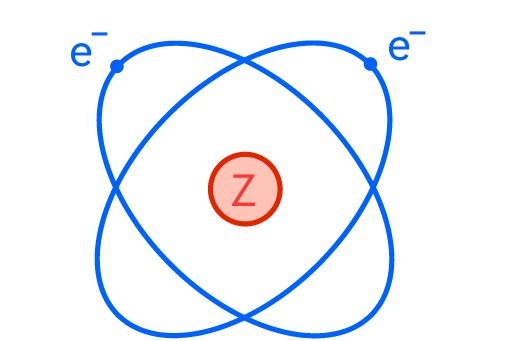
\includegraphics[width=\linewidth]{images/l11_1(1).jpeg}
	\end{subfigure}
	\hfill                          
	\begin{subfigure}{0.45\textwidth} 
		\centering
		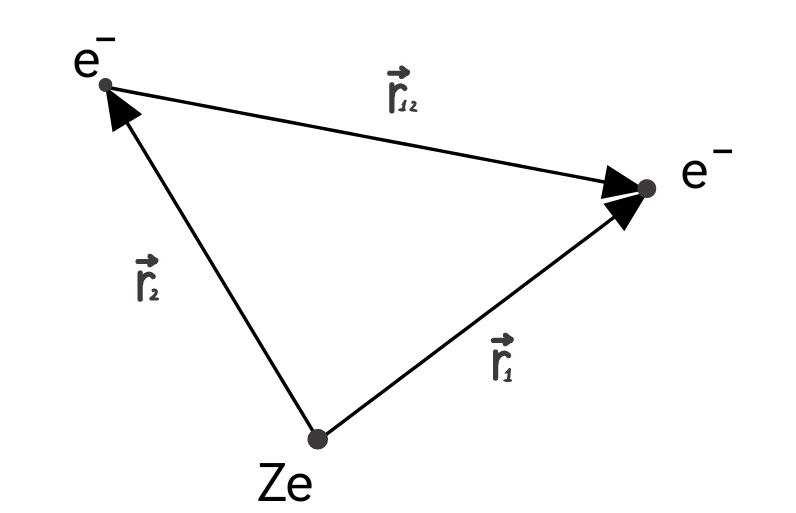
\includegraphics[width=\linewidth]{images/l11_2(1).jpeg}
	\end{subfigure}
\end{figure}
Рассмотрим атом гелия с зарядом ядра $Z = 2$ (2 протона + 2 нейтрона), вокруг которого вращается два тождественных электрона. Пусть радиус-вектор от ядра до одного электрона --- $\vec{r}_1$, а до другого --- $\vec{r}_2$.
\[
\vec{r}_{12} = \vec{r}_1 - \vec{r}_2, \ r_{12} = |\vec{r}_{12}|
\]

Пусть $\hat{H}_1$ и $\hat{H}_2$ --- невозмущенные гамильтонианы электронов, взаимодействующих с ядром (но не друг с другом). Тогда в координатном представлении
\[
\braupket{\vec{r}_1,~\vec{r}_2}{\hat{H}_1 + \hat{H}_2 + \hat{V}_{12}}{\psi} = E\psi(\vec{r}_1,~\vec{r}_2)
\]
Вспомним, что
\[
\braupket{\vec{r}_i}{\hat{H}_i}{\varphi} = \left(-\dfrac{\hbar^2}{2m}\Delta_i - Z\dfrac{e^2}{r_i}\right)\varphi(\vec{r}_i)
\]
Тогда
\[
\left(-\dfrac{\hbar^2}{2m}(\Delta_1 + \Delta_2)-Z\dfrac{e^2}{r_1}-Z\dfrac{e^2}{r_2} \right)\psi(\vec{r}_1,~\vec{r}_2) = E\psi(\vec{r}_1,~\vec{r}_2)
\]
\[
\Longrightarrow \braupket{\vec{r}_1,~\vec{r}_2}{\hat{V}_{12}}{\psi} = \dfrac{e^2}{r_{12}}\psi(\vec{r}_1,~\vec{r}_2)
\]
Для невозмущенного гамильтониана
\[
\braupket{\vec{r}_1,~\vec{r}_2}{\hat{H}_0}{\psi} = \left(-\dfrac{\hbar^2}{2m}(\Delta_1 + \Delta_2)-Z\dfrac{e^2}{r_1}-Z\dfrac{e^2}{r_2}\right)\psi^{(0)}(\vec{r}_1,~\vec{r}_2) = E^{(0)}\psi^{(0)}(\vec{r}_1,~\vec{r}_2)
\]
Т.к. электроны не взаимодействуют
\[
\psi^{(0)}(\vec{r}_1,~\vec{r}_2) = \psi_{n_1~l_1~l_{1z}}^{(0)}(\vec{r}_1)\psi_{n_2~l_2~l_{2z}}^{(0)}
\]